\documentclass[12pt]{article}
\usepackage[utf8]{inputenc}
\usepackage[margin=1in]{geometry}
\usepackage{graphicx}
\usepackage{setspace}
\usepackage{biblatex}
\addbibresource{Zotero.bib}
\usepackage{hyperref}
\hypersetup{colorlinks=true,urlcolor=cyan,citecolor=black}
\urlstyle{same}
\doublespacing

\begin{document}
\begin{center}
\Huge Virtual Reality
\end{center}

Virtual reality is anticipated to be the ``next big thing" of our near future. \cite{baruahVirtualRealityVRTK42020} Despite the futuristic perception it incites, the future of virtual reality goes all the way back to the 1920's. \cite{grasnickBasicsVirtualReality2021a} It is fascinating to see the evolution of the designs used throughout the decades until the one currently used. After covering the history of VR, a basic understanding of how modern-day headsets reasonably follows. However, before this, it is necessary to cover the basic terminology used to describe virtual reality and its related technology.

To start, it is important to understand the difference between virtual reality (VR), augmented reality (AR), mixed reality (MR), and extended reality (XR). Also, for the sake of clarification, it is convenient to refer to the real world as external reality (ER). An easy way to clarify between these terms is with visual graphics. Virtual Reality is the experience of being in a reality completely isolated from external reality. This includes not only fake worlds created virtually, but even replications of external, real places, provided it is only a replication. The graphic below helps illustrate this point, where the virtual reality is completely exclusive of actual reality. An example of this includes the HTC Vive VR Headset.

\begin{center}
\centering
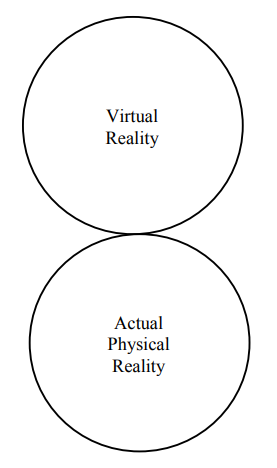
\includegraphics[width = 5cm]{Image A.png}

Virtual Reality
\cite{vermaAdvancesAugmentedReality2022a}
\end{center}

Augmented reality, on the other hand, is virtually altering or adding on to the external world. In terms of its graphical representation, we see the external reality fully encapsulated in the larger augmented reality, since augmented reality is based off external reality with virtual additions or alterations. This is the least computationally intensive between virtual reality, augmented reality, and mixed reality. An example of this is seen with Pokémon GO, where the game adds its features onto the real world.

\begin{center}
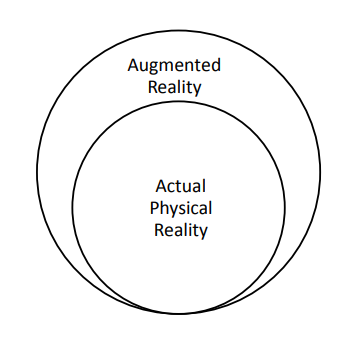
\includegraphics[width = 5cm]{Image B.png}

Augmented Reality
\cite{vermaAdvancesAugmentedReality2022a}
\end{center}

Mixed reality, as the name hints, is simply a mixing of virtual reality and augmented reality. Essentially, the goal of mixed reality is to make the aspects of the real world indistinguishable from those that are virtual and allowing full interaction between both. This is the most computationally intensive of VR, AR, and MR due to the complexity involved in replicating the interactivity between virtual and external objects.
\cite{vermaAdvancesAugmentedReality2022a}

\begin{center}
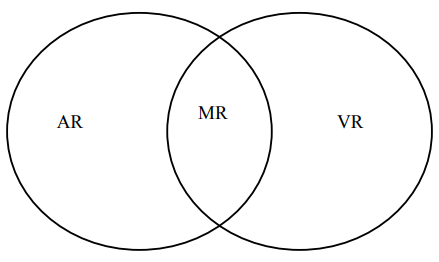
\includegraphics[width = 5cm]{Image C.png}

Mixed Reality
\cite{vermaAdvancesAugmentedReality2022a}
\end{center}

Extended reality is not another new category like three other terms. Extended reality, rather is less a distinct category of its own and more just a grouping of all virtual reality, augmented reality, and mixed reality. It also includes any new related technologies in the future. \cite{vermaAdvancesAugmentedReality2022a}

\begin{center}
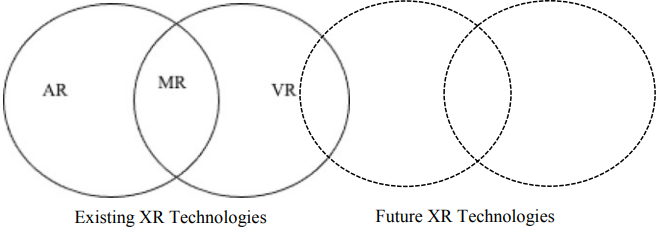
\includegraphics[width = 8cm]{Image D.png}

Extended Reality
\cite{vermaAdvancesAugmentedReality2022a}
\end{center}


Virtual reality has been attempted with a few different approaches. The most popular approach was called stereoscopy, which, strictly speaking, is the use of duplicate images to display a 3D image. Stereoscopes are the devices we typically associate virtual reality to, such as the Oculus Rift, where the device consists of a binocular-like headset with separate images for each eye. 

The issue with stereoscopy is that it is restricted to sight and hearing. In his four laws of cinematic art, Morton Heilig (1950's film artist, inventor, and virtual reality pioneer) estimates, sight accounts for about 70\% and hearing for about 20\% of what our combined five senses capture. While these values are clearly approximations, it leads us to wonder if true virtual reality can ever be achieved with stereoscopy. Heilig himself attempted this, creating an environment-simulator, which included full 3D vision and sound, but also included minor smell and feeling sensation. While the device itself had a somewhat awkward design, it included a headset piece which would ultimately inspire the future design of VR headsets. While the thought of virtual reality using all five senses has proven to be impractical, if not, impossible, the idea has been talked about for nearly a century. In 1930, author Stanley Weinbaum created a fictional short story, called ``Pygmalion’s Spectacles,” where a strange scientist, Professor Ludwig, creates a spectacle-like device which uses electricity and chemicals to replicate the experience of a dream. In much more recent times, the ``Matrix" movies revived the idea of fully captivating all five senses in an artificial reality. While we may never get to a point where we can use the full potential of our senses in an augmented reality (which, considering Weinbaum's strange story about simulating the experience of a dream or the idea behind the ``Matrix", might likely be for the best), it is interesting to see what is in store for expected near future of virtual reality, especially in regard to gaming.
\cite{grasnickBasicsVirtualReality2021a}

The main reason for virtual reality taking so long to grow in popularity, considering that the idea has been out for roughly a century, is due to the fact that all the necessary technology for it is only finally becoming available. 




The idea behind how virtual reality works is fairly simple, but the execution is difficult. ``Faster, cheaper, more powerful technology has pushed the boundaries of VR beyond what has been known because drawing three-dimensional objects to a screen up to, and in some cases past, 100 times a second is a computationally intensive process."
\cite{baruahVirtualRealityVRTK42020} VR works first by using some means of tracking the user's motion. ``In VR headsets that have sensors embedded in them for head tracking, something known as six degrees of freedom, or 6DOF, is the concept used to make head tracking work. This system basically plots your head in an XYZ plane, and measures head movements by forward, backward, side to side, and yaw and roll."
\cite{ThisEngineeringHow2020}
\begin{center}
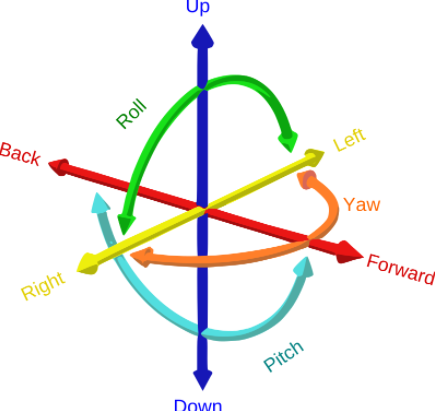
\includegraphics[width = 5cm]{Image E.png}

The Six Directions of Freedom
\cite{SixDegreesFreedom}
\end{center} Virtual Reality Headsets use several types of devices to detect these six degrees of freedom, from gyroscopes, accelerometers, magnetometers, to even external LED's detected by sensors. \cite{ThisEngineeringHow2020}
Now that the full scope of motion is detectable, the other task that needs completed is adding perspective. The virtual reality headsets use two separate images for each eye to account for the slightly different perspectives from each eye, which gives us the feeling of being in 3D instead of just seeing a flat image in front of us.  Finally, to keep track of where you are in the virtual world, virtual reality systems use quaternions. Quaternion notation, invented by Hamilton, allows us to remember relative position from a point in three dimensions with rotation. Using the position-sensing devices along with the use of quaternions, virtual reality systems can detect the movement made by the headset and account for it in the virtual world, adjusting the perspective. \cite{grasnickBasicsVirtualReality2021a}

Now that our technology is becoming advanced enough to handle the intense computational power necessary to run it, virtual reality very well could be as impactful in the near future as anticipated. It is incredible to realize that the first attempts at it go back a hundred years, and how the current design is based off a design from the 1960's. \cite{grasnickBasicsVirtualReality2021a} However, knowing how momentous virtual reality currently is, it is perhaps more captivating to explore the basics of how the modern-day technology works. Whether or not it really lives up to its hype, virtual reality is undoubtedly one of the most fascinating topics of current time.

\pagebreak
\medskip
\printbibliography[heading=bibintoc ,title={Works Cited}]
\end{document}